% LaTeX source for ``การเรียนรู้ของเครื่องสำหรับเคมีควอนตัม (Machine Learning for Quantum Chemistry)''
% Copyright (c) 2022 รังสิมันต์ เกษแก้ว (Rangsiman Ketkaew).

% License: Creative Commons Attribution-NonCommercial-NoDerivatives 4.0 International (CC BY-NC-ND 4.0)
% https://creativecommons.org/licenses/by-nc-nd/4.0/

\chapter{การเรียนรู้เชิงลึก}
\label{ch:dl}

เอาล่ะครับในบทนี้เราจะมาดูหัวข้อการเรียนรู้ลึกหรือ Deep Learning ซึ่งเป็นหนึ่งในคำศัพท์ Buzzword ที่หลาย ๆ คนต่างก็พูดถึงในช่วงระยะเวลา
10 ปีที่ผ่านมา ไม่ว่าจะเป็นวงการอาชีพไหน ๆ ก็จะต้องมีการนำ Deep Learning ไปใช้ทั้งนั้น และแน่นอนว่าหนึ่งในนั้นก็คือการนำ Deep Learning 
มาประยุกต์ใช้ในงานวิจัยทางด้านเคมี ซึ่งข้อมูลที่นักเคมีมีอยู่ในมือนั้นมากมายมหาศาล ดังนั้นจึงน่าสนใจว่า Deep Learning จะช่วยนักเคมีในการขับเคลื่อน%
งานวิจัยได้อย่างไร

ในบทก่อนหน้านี้นั้นเราได้พูดถึง Supervised Learning กันไปแล้ว ซึ่งจะเป็นการทำนายค่า $y$ จากข้อมูลนำเข้า $x$ โดยเป็นการพิจารณาในกรณี%
ของการถดถอยเชิงเส้น ในลำดับถัดมา (ซึ่งก็คือในบทนี้) เราจะมาพิจารณากรณีที่พารามิเตอร์ของเรานั้นมีความไม่เป็นเชิงเส้น (Nonlinear) กันครับ
ซึ่งโมเดลปัญญาประดิษฐ์ที่ถูกนำมาใช้อย่างแพร่หลายนั้นก็คือ Neural Network นั่นเอง แต่ว่าอย่าเพิ่งสับสนกับคำศัพท์ระหว่าง Neural Network กับ
Deep Learning นะครับ เพราะว่าจริง ๆ แล้วทั้งสองคำนี้ก็มีความเชื่อมโยงกัน ซึ่ง Deep Learning นั้นถือว่าเป็น Neural Network นั่นเอง

%--------------------------
\section{การเรียนรู้ของโมเดลที่ไม่เป็นเชิงเส้น}
\label{sec:nonlinear_ml}
\idxboth{การเรียนรู้ของโมเดลที่ไม่เป็นเชิงเส้น}{Nonlinear Supervised Learning}
%--------------------------

สมมติว่าเรามี $\{(x^{(i)}, y^{(i)})\}^n_{i=1}$ ซึ่งเป็นตัวอย่างชุดข้อมูลฝึกสอน (Training Data) และเราจะเริ่มกันด้วยกรณีที่ง่ายที่สุด%
นั่นก็คือ $y^{(i)} \in \mathbb{R}$ และ $h_\theta(x) \in \mathbb{R}$ 

เราจะทำการกำหนด Cost/Loss Function ขึ้นมา ซึ่งเราจะใช้ Least Square Cost function สำหรับข้อมูลลำดับที่ $i$ นั่นก็คือคู่อันดับ 
$(x^{(i)} ,y^{(i)} )$ ดังนี้ 

\begin{equation}\label{eq:loss}
    J^{(i)} (\theta) = \frac{1}{2} \left(h_\theta (x^{(i)}) - y^{(i)}\right)^2
\end{equation}

\noindent และกำหนด Mean-Square Cost Function สำหรับชุดข้อมูลดังนี้

\begin{equation}\label{eq:mse_loss}
    J(\theta) = \frac 1 n \sum_{i=1}^n J^{(i)}(\theta)
\end{equation}

\noindent ซึ่งผู้อ่านอาจจะสังเกตได้ว่าสมการข้างต้นนั้นจะเหมือนกับในกรณีของ Linear Regression เว้นแต่จะต่างกันตรงที่เราได้มีการเพิ่ม $1/n$
เข้าไปในด้านหน้าของ Cost Function \footnote{การคูณ Cost Function ด้วยปริมาณสเกลาร์ เช่น ตัวเลข จะไม่ทำให้จุดต่ำสุดสัทพันธ์ 
(Local minima) และจุดต่ำสุดสัมบูรณ์ (Global Minima) เปลี่ยนไป} นอกจากนี้ผู้อ่านจะต้องทำความเข้าใจด้วยว่าการปรับค่าพารามิเตอร์ 
(Parameterization) ของ $h_\theta(x)$ นั้นจะแตกต่างจากกรณีของ Linear Regression ถึงแม้ว่าเราจะใช้ Cost Function ที่เหมือน%
กันก็ตาม 

ลำดับถัดมาคือตัวปรับค่าพารามิเตอร์ (Optimizer) ซึ่งโดยทั่วไปแล้วเรามักจะใช้ Stochastic Gradient Descent (SGD) นั่นก็เพราะว่าเป็นวิธีที่%
ง่ายและไม่ซับซ้อนสำหรับการปรับค่าให้เหมาะสม (Optimize) Loss Function ของเราซึ่งเขียนแทนด้วย $J(\theta)$ ซึ่งการปรับค่านั้นจะใช้%
สมการดังต่อไปนี้\footnote{สังเกตว่าเราใช้เครื่องหมาย $a := b$ เพื่อบ่งบอกการดำเนินการ (Operation) ซึ่งเป็นการระบุค่าให้กับตัวแปรใน%
โปรแกรมคอมพิวเตอร์}

\begin{equation}
    \theta := \theta - \alpha\nabla_\theta J(\theta)
\end{equation}

\noindent โดยที่ $\alpha$ คืออัตราเร็วในการเรียนรู้ \textit{Learning Rate} หรืออาจจะเรียกว่า \textit{Step Size} ก็ได้ 
โดยเรามักจะกำหนดให้ค่า $\alpha$ มีค่ามากกว่าศูนย์ ด้านล่างคืออัลกอริทึมของ SGD

\begin{algorithm}[ht]
    \caption{อัลกอริทึมของ Stochastic Gradient Descent}
    \label{alg:sgd_dl}
    \begin{algorithmic}
    \State Hyperparameter: learning rate $\alpha$, number of total iteration $n_\text{iter}$.
    \State Initialize $\theta$ randomly.
    \For{$i = 1$ to $n_\text{iter}$}
        \State Sample $j$ uniformly from ${1,\ldots,n}$, and update $\theta$ by
        \begin{equation*}
            \theta := \theta - \alpha\nabla_\theta J^{(j)}(\theta)
        \end{equation*}
    \EndFor
    \end{algorithmic}
\end{algorithm}

ในทางปฏิบัตินั้นการคำนวณ Gradient ของ $B$ หลาย ๆ ครั้งสามารถทำพร้อมกันได้เพราะว่าในปัจจุบันเรามีเทคนิคการทำการคำนวณแบบขนาน 
(Parallelization) สำหรับการปรับค่า $\theta$ ซึ่งจะเร็วกว่าการคำนวณ Gradient ของ $B$ แบบแยกกันทีละค่าแน่นอน ซึ่งการที่เราจะทำ%
การคำนวณแบบพร้อม ๆ กันได้นั้นเราจะต้องมีการแบ่ง Data ของเราออกเป็นส่วนย่อย ๆ แล้วทำการคำนวณแยกกัน (Batch) ซึ่งเราจะต้องมีการปรับ%
อัลกอริทึมเล็กน้อย โดยด้านล่างคืออัลกอริทึมของ Mini-batch SGD ซึ่งได้จากการปรับอัลกอริทึมของ SGD แบบธรรมดา  

\begin{algorithm}[ht]
    \caption{Mini-batch stochastic gradient descent}
    \label{alg:sgd_minibatch}
    \begin{algorithmic}
    \State Hyperparameter: learning rate $\alpha$, batch size $B$, \# iteration $n_\text{iter}$.
    \State Initialize $\theta$ randomly.
    \For{$i = 1$ to $n_\text{iter}$}
        \State Sample $j$ uniformly from ${1,\ldots,n}$, and update $\theta$ by
        \State Sample $B$ examples $j_1,\ldots,j_B$ (without replacement) uniformly from $\{1,\ldots,n\}$, 
        and update $\theta$ by
        \begin{equation*}
            \theta := \theta - \frac{\alpha}{B}\sum_{k=1}^B\nabla_\theta J^{(j_k)}(\theta)
        \end{equation*}
    \EndFor
    \end{algorithmic}
\end{algorithm}

โดยทั่วไปแล้วโมเดล Deep Learning นั้นจะมีการเรียนรู้ซึ่งอาศัยอัลกอริทึมตามด้านบนโดยทำตามขั้นตอนดังต่อไปนี้

\begin{enumerate}
    \item กำหนด $h_\theta(x)$
    \item เขียนอัลกอริทึม Backpropagation เพื่อคำนวณ Gradient ของ Loss Function $J^{(j)}(\theta)$
    \item ทำการปรับ Loss Function โดยใช้ SGD หรือ Mini-batch SGD หรือใช้ Optimizer ตัวอื่น ๆ
\end{enumerate}

%--------------------------
\section{โครงข่ายประสาทเทียม}
\label{sec:nn}
\idxboth{โครงข่ายประสาทเทียม}{Neural Network}
%--------------------------

โครงข่ายประสาทเทียม (Neural Network)

การเรียนรู้เชิงลึกรูปแบบที่มาตรฐานที่สุดคือการเรียนรู้แบบมีผู้สอนด้วยโมเดลแบบไม่เป็นเชิงเส้น (Supervised learning with nonlinear model)

%--------------------------
\section{การแผร่กระจายการเรียนรู้}
\idxboth{การแผร่กระจายการเรียนรู้}{Learning Propagation}
%--------------------------

การแผร่กระจายการเรียนรู้ (Learning Propagation) เป็นขั้นตอนการเรียนรู้ของโมเดล Neural Network ที่เลียนแบบการทำงานของสมอง 


\begin{center}
\begin{tikzpicture}[x=2.2cm,y=1.4cm]
    \message{^^JNeural network with arrows}
    \readlist\Nnod{4,5,5,5,3} % array of number of nodes per layer
    
    \message{^^J  Layer}
    \foreachitem \N \in \Nnod{ % loop over layers
    \edef\lay{\Ncnt} % alias of index of current layer
    \message{\lay,}
    \pgfmathsetmacro\prev{int(\Ncnt-1)} % number of previous layer
    \foreach \i [evaluate={\y=\N/2-\i; \x=\lay; \n=\nstyle;}] in {1,...,\N}{ % loop over nodes
    
    % NODES
    \node[node \n] (N\lay-\i) at (\x,\y) {$a_\i^{(\prev)}$};
    %\node[circle,inner sep=2] (N\lay-\i') at (\x-0.15,\y) {}; % shifted node
    %\draw[node] (N\lay-\i) circle (\R);
    
    % CONNECTIONS
    \ifnum\lay>1 % connect to previous layer
    \foreach \j in {1,...,\Nnod[\prev]}{ % loop over nodes in previous layer
    \draw[connect arrow] (N\prev-\j) -- (N\lay-\i); % connect arrows directly
    %\draw[connect arrow] (N\prev-\j) -- (N\lay-\i'); % connect arrows to shifted node
    }
    \fi % else: nothing to connect first layer
    
    }
    
    }
    
    % LABELS
    \node[above=5,align=center,mygreen!60!black] at (N1-1.90) {input\\[-0.2em]layer};
    \node[above=2,align=center,myblue!60!black] at (N3-1.90) {hidden layers};
    \node[above=8,align=center,myred!60!black] at (N\Nnodlen-1.90) {output\\[-0.2em]layer};
    
    \end{tikzpicture}
\end{center}

%--------------------------
\subsection{การแผ่กระจายแบบไปข้างหน้า}
\label{sec:forward_prop}
\idxboth{การแผ่กระจายแบบไปข้างหน้า}{Forward Propagation}
%--------------------------

ในขั้นเริ่มต้นของการฝึกสอนโมเดล Neural Network นั้น โมเดลจะยังไม่มีพารามิเตอร์ที่ถูกต้อง ดังนั้นเราจึงต้องสุ่มค่าเริ่มต้นของพารามิเตอร์ขึ้นมาก่อน
หลังจากนั้นจึงทำ Forward Propagation รอบที่หนึ่งแล้วก็เปรียบเทียบผลการทำนายกับคำตอบ ($Output$) ที่โมเดลทราบก่อนหน้านั้นแล้ว
ขั้นตอนต่อมาคือการปรับพารามิเตอร์ที่สำคัญอีกสองตัวนั่นคือน้ำหนัก (Weight) และความอคติหรือความโน้มเอียง (Bias) ให้มีค่าที่ถูกต้อง ซึ่งใน%
ขั้นตอนนี้เราจะใช้กระบวนการที่ตรงข้ามกันเรียกว่า Backward propagation โดยการทำ Propagation ทั้งสองแบบพร้อม ๆ กันครบหนึ่งรอบนั้น%
จะเรียกว่า 1 Epoch แต่ต้องระวังนะครับว่า Epoch, Batch Size และ Iteration นั้นมีความหมายต่างกัน โดยความแตกตางมีดังนี้

\begin{description}[font=$\bullet$~\normalfont\scshape\bfseries\color{red!50!black}]
    \item[1 Epoch] การทำ Forward และ Backward Propagation 1 ครั้ง
    \item[Batch Size] จำนวนของข้อมูลที่ใช้ในการฝึกสอนในการทำ Forward และ Backward Propagation 1 รอบ
    \item[Iteration] จำนวนของรอบในการฝึกสอน ซึ่งแต่ละรอบจะใช้ Batch Size ที่ถูกกำหนดไว้ก่อนการฝึกสอน
\end{description}

เพื่อให้เห็นภาพมากขึ้น เราลองมาดูตัวอย่างกัน เช่น ถ้าเรามีจำนวนข้อมูลในการฝึกสอน 1000 ตัวอย่างและกำหนด Batch Size เป็น 500 จะได้ว่าโมเดลของเรา%
จะใช้ 2 Iterations สำหรับการฝึกสอน 1 Epoch

%--------------------------
\subsection{การแผ่กระจายแบบย้อนกลับ}
\label{sec:backprop}
\idxboth{การแผ่กระจายแบบย้อนกลับ}{Backpropagation}
%--------------------------

การแผ่กระจายแบบย้อนกลับ (Backpropagation)

%--------------------------
\section{ฟังก์ชันกระตุ้น}
\label{sec:act_func}
\idxboth{ฟังก์ชันกระตุ้น}{Activation Function}
%--------------------------

ฟังก์ชันกระตุ้น (Activation Function)

%--------------------------
\section{ฟังก์ชันความคลาดเคลื่อน}
\label{sec:loss_func}
\idxboth{ฟังก์ชันความคลาดเคลื่อน}{Loss Function}
%--------------------------

ฟังก์ชันความคลาดเคลื่อน (Loss Function หรือ Cost Function หรือ Error Function)

\begin{equation}
    \text{MAE} = \frac{1}{n} \sum_{i=1}^{n} | \tilde{x}_{i} - x_{i} |
\end{equation}

\begin{equation}
    \text{MAPE} = \frac{1}{n} \sum_{i=1}^{n} \left| \frac{\tilde{x}_{i} - x_{i}}{x_{i}} \right| \times 100
\end{equation}

\begin{equation}
    \text{MSE} = \frac{1}{n} \sum_{i=1}^{n} \left( \tilde{x}_{i} - x_{i} \right)^2
\end{equation}

\begin{equation}
    \text{MaxAE} = max\{\tilde{x}_{i} - x_{i}\}, i = 1, 2, ..., n
\end{equation}

\begin{equation}
    \text{MaxAPE} = max\left\{\left| \frac{\tilde{x}_{i} - x_{i}}{x_{i}} \right| \times 100 \right\}, i = 1, 2, ..., n
\end{equation}

\begin{equation}
    \text{RMSD} = \sqrt{ \frac{1}{n} \sum_{i=1}^{n} (\tilde{x}_{i} - x_{i})^{2} }
    \label{eq:rmsd}
\end{equation}

\begin{equation}
    \text{GRMSD} = \sqrt[2n]{ \prod_{i=1}^{n} (\tilde{x}_{i} - x_{i})^{2} }
    \label{eq:grmsd}
\end{equation}

\begin{equation}
    \text{GWRMSD} = \sqrt{ \frac{\sum_{i=1}^{n} \zeta_{i} (\tilde{x}_{i} - x_{i})^{2}}{\sum_{i=1}^{n} \zeta_{i} } }
    \label{eq:gwrmsd}
\end{equation}

\indent โดยที่

\begin{equation}
    \zeta_{i} = e^{-(\tilde{x}_{i} - x_{i}) / c}
\end{equation}

%--------------------------
\section{ตัวปรับความเหมาะสม}
\label{sec:optimizer}
\idxboth{ตัวปรับความเหมาะสม}{Optimizer}
%--------------------------

ตัวปรับความเหมาะสมหรือปรับประสิทธิภาพการเรียนรู้ของโมเดล (Optimizer)

%--------------------------
\section{สถาปัตยกรรมของโครงข่ายประสาท}
\label{sec:architecture}
\idxboth{สถาปัตยกรรมของโครงข่ายประสาท}{Neural Network Architecture}
%--------------------------

สถาปัตยกรรมของโครงข่ายประสาทเทียม (Architecture)

%--------------------------
\section{ตัวอย่างการสร้างและฝึกสอนโมเดลด้วย TensorFlow}
%--------------------------

ในหัวข้อนี้จะเป็นการยกตัวอย่างประกอบโค้ดของการสร้างและฝึกสอนโมเดลในการทำนายค่าสภาพการละลายของโมเดล ซึ่งค่าสภาพการละลายหรือ
Solubility เป็นความสามารถของสสารในการละลายในน้ำ ยิ่งมีค่าเยอะหมายความว่าสสารนั้นยิ่งละลายในน้ำได้ดี โดยเราจะใช้ Module Keras 
ซึ่งเป็น Library ที่ถูกติดตั้งและพัฒนาให้เป็น API ของ TensorFlow ในการสร้างโมเดล
\footnote{ดูรายละเอียดของ Keras ได้ที่ \url{https://keras.io/guides/sequential_model/}}

\begin{enumerate}
\item ขั้นตอนแรกเราจะต้องทำการกำหนดรายละเอียดของ Neural Network

\begin{lstlisting}[style=MyPython]
import numpy as np
import tensorflow as tf

# our hidden layer
# We only need to define the output dimension - 32.
hidden_layer = tf.keras.layers.Dense(32, activation="tanh")
# Last layer - which we want to output one number
# the predicted solubility.
output_layer = tf.keras.layers.Dense(1)

# Now we put the layers into a sequential model
model = tf.keras.Sequential()
model.add(hidden_layer)
model.add(output_layer)
\end{lstlisting}

\vspace{1em}

\item ทำการทดสอบโดยเรียกใช้โมเดลเพื่อแสดงข้อมูลของสสารสามตัวแรกในชุดข้อมูล

\begin{lstlisting}[style=MyPython]
# Try out our model on first few datapoints
model(soldata[feature_names].values[:3])

# Output
<tf.Tensor: shape=(3, 1), dtype=float32, numpy=
array([[ 0.18162721],
        [-0.416314  ],
        [-0.32956678]], dtype=float32)>
\end{lstlisting}

\vspace{1em}

\item คอมไพล์โมเดล

\begin{lstlisting}[style=MyPython]
model.compile(optimizer="SGD", loss="mean_squared_error")
\end{lstlisting}

\vspace{1em}

\item ฝึกสอนโมเดล

\begin{lstlisting}[style=MyPython]
model.fit(train_data, epochs=50)
\end{lstlisting}

\vspace{1em}

\item ทำนายค่าความสามารถในการละลายของโมเลกุล

\begin{lstlisting}[style=MyPython]
yhat = np.squeeze(model.predict(test_data))
test_y = soldata["Solubility"].values[:test_N]
\end{lstlisting}

\vspace{1em}

\item พลอตกราฟเปรียบเทียบค่าสภาพการละลายที่ได้จากการทำนายและค่าอ้างอิง

\begin{lstlisting}[style=MyPython]
plt.plot(test_y, yhat, ".")
plt.plot(test_y, test_y, "-")
plt.xlabel("Measured Solubility $y$")
plt.ylabel("Predicted Solubility $\hat{y}$")
plt.text(
    min(test_y) + 1,
    max(test_y) - 2,
    f"correlation = {np.corrcoef(test_y, yhat)[0,1]:.3f}",
)
plt.text(
    min(test_y) + 1,
    max(test_y) - 3,
    f"loss = {np.sqrt(np.mean((test_y - yhat)**2)):.3f}",
)
plt.show()
\end{lstlisting}

\noindent ได้กราฟดังต่อไปนี้

\begin{figure}[H]
    \centering
    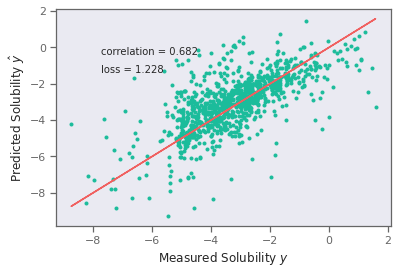
\includegraphics[width=0.8\linewidth]{fig/predict_solubility.png}
    \caption{เปรียบเทียบค่าสภาพการละลายที่ได้จากการทำนายและค่าอ้างอิง}
    \label{fig:krr_gpr}
\end{figure}

\end{enumerate}
